\documentclass[letterpaper, 10 pt, conference]{ieeeconf}

\IEEEoverridecommandlockouts
\overrideIEEEmargins

\usepackage[utf8]{inputenc}
\usepackage[T1]{fontenc}
\usepackage{graphicx}
\usepackage{amsmath}
\usepackage{amssymb}
\usepackage{url}

% report_numbers.tex — auto-generated by scripts/run_phase_8_report_tables.py
% DO NOT EDIT BY HAND — regenerate with: make phase8
%
% Usage in report preamble:  % report_numbers.tex — auto-generated by scripts/run_phase_8_report_tables.py
% DO NOT EDIT BY HAND — regenerate with: make phase8
%
% Usage in report preamble:  % report_numbers.tex — auto-generated by scripts/run_phase_8_report_tables.py
% DO NOT EDIT BY HAND — regenerate with: make phase8
%
% Usage in report preamble:  \input{../artifacts/tables/report_numbers}

% Seeds
\newcommand{\SeedList}{42, 43, 44, 45, 46}
\newcommand{\NumSeeds}{5}

% Phase 1 — environment models
\newcommand{\CPNStates}{864}
\newcommand{\CPModelBuildWallClock}{36.6}
\newcommand{\BJNStates}{290}

% Phase 2 — Blackjack VI / PI
\newcommand{\BJVIIters}{9}
\newcommand{\BJVIWallClock}{0.001}
\newcommand{\BJVIReturn}{-0.0288}
\newcommand{\BJVIReturnIQR}{0.023}
\newcommand{\BJPIIters}{3}
\newcommand{\BJPIWallClock}{0.001}
\newcommand{\BJPIReturn}{-0.0288}
\newcommand{\BJPIReturnIQR}{0.023}
\newcommand{\BJVIPolicyMatch}{100.0\%}

% Phase 3 — CartPole VI / PI (default grid unless noted)
\newcommand{\CPCoarseNStates}{72}
\newcommand{\CPCoarseCoverage}{89.6\%}
\newcommand{\CPCoarseVIIters}{1376}
\newcommand{\CPCoarseVIWallClock}{0.009}
\newcommand{\CPCoarseVIEpLen}{500.0}
\newcommand{\CPCoarseVIEpLenIQR}{0.00}
\newcommand{\CPCoarsePIIters}{9}
\newcommand{\CPCoarsePIWallClock}{0.136}
\newcommand{\CPCoarsePIEpLen}{500.0}
\newcommand{\CPCoarsePIEpLenIQR}{0.00}
\newcommand{\CPCoarsePolicyAgreement}{100.0\%}
\newcommand{\CPDefaultNStates}{864}
\newcommand{\CPDefaultCoverage}{25.2\%}
\newcommand{\CPDefaultVIIters}{1376}
\newcommand{\CPDefaultVIWallClock}{0.588}
\newcommand{\CPDefaultVIEpLen}{456.8}
\newcommand{\CPDefaultVIEpLenIQR}{5.36}
\newcommand{\CPDefaultPIIters}{10}
\newcommand{\CPDefaultPIWallClock}{0.551}
\newcommand{\CPDefaultPIEpLen}{465.5}
\newcommand{\CPDefaultPIEpLenIQR}{1.97}
\newcommand{\CPDefaultPolicyAgreement}{98.4\%}
\newcommand{\CPFineNStates}{4000}
\newcommand{\CPFineCoverage}{16.3\%}
\newcommand{\CPFineVIIters}{1376}
\newcommand{\CPFineVIWallClock}{16.291}
\newcommand{\CPFineVIEpLen}{434.9}
\newcommand{\CPFineVIEpLenIQR}{3.42}
\newcommand{\CPFinePIIters}{12}
\newcommand{\CPFinePIWallClock}{50.474}
\newcommand{\CPFinePIEpLen}{436.7}
\newcommand{\CPFinePIEpLenIQR}{3.00}
\newcommand{\CPFinePolicyAgreement}{99.0\%}

% Phase 4 — Blackjack SARSA / Q-Learning
\newcommand{\BJSarsaControlledReturn}{-0.0406}
\newcommand{\BJSarsaControlledReturnIQR}{0.028}
\newcommand{\BJSarsaControlledWinRate}{0.437}
\newcommand{\BJSarsaControlledConvEp}{179,525}
\newcommand{\BJSarsaControlledConvIQR}{188,675}
\newcommand{\BJQLControlledReturn}{-0.0546}
\newcommand{\BJQLControlledReturnIQR}{0.028}
\newcommand{\BJQLControlledWinRate}{0.429}
\newcommand{\BJQLControlledConvEp}{230,625}
\newcommand{\BJQLControlledConvIQR}{234,175}
\newcommand{\BJSarsaTunedReturn}{-0.0364}
\newcommand{\BJSarsaTunedReturnIQR}{0.047}
\newcommand{\BJSarsaTunedWinRate}{0.437}
\newcommand{\BJSarsaTunedConvEp}{66,825}
\newcommand{\BJSarsaTunedConvIQR}{54,725}
\newcommand{\BJQLTunedReturn}{-0.0538}
\newcommand{\BJQLTunedReturnIQR}{0.021}
\newcommand{\BJQLTunedWinRate}{0.430}
\newcommand{\BJQLTunedConvEp}{162,800}
\newcommand{\BJQLTunedConvIQR}{151,000}
\newcommand{\BJMFTrainWallClock}{84.7}

% Phase 5 — CartPole SARSA / Q-Learning
\newcommand{\CPSarsaControlledEpLen}{275.6}
\newcommand{\CPSarsaControlledEpLenIQR}{325.7}
\newcommand{\CPSarsaControlledConvEp}{1,160}
\newcommand{\CPSarsaControlledConvIQR}{600}
\newcommand{\CPQLControlledEpLen}{326.8}
\newcommand{\CPQLControlledEpLenIQR}{309.1}
\newcommand{\CPQLControlledConvEp}{1,140}
\newcommand{\CPQLControlledConvIQR}{600}
\newcommand{\CPSarsaTunedEpLen}{325.3}
\newcommand{\CPSarsaTunedEpLenIQR}{323.7}
\newcommand{\CPSarsaTunedConvEp}{880}
\newcommand{\CPSarsaTunedConvIQR}{100}
\newcommand{\CPQLTunedEpLen}{376.8}
\newcommand{\CPQLTunedEpLenIQR}{169.1}
\newcommand{\CPQLTunedConvEp}{1,180}
\newcommand{\CPQLTunedConvIQR}{600}
\newcommand{\CPMFTrainWallClock}{400.4}
\newcommand{\CPDiscWallClock}{557.1}
% Phase 5 — CartPole discretization study
\newcommand{\CPDiscCoarseSarsaEpLen}{364.3}
\newcommand{\CPDiscCoarseQLEpLen}{438.1}
\newcommand{\CPDiscDefaultSarsaEpLen}{325.3}
\newcommand{\CPDiscDefaultQLEpLen}{376.8}
\newcommand{\CPDiscFineSarsaEpLen}{94.6}
\newcommand{\CPDiscFineQLEpLen}{110.3}

% Phase 6 — wall-clock summary
\newcommand{\BJVIWallClockPhaseSix}{0.001}
\newcommand{\BJPIWallClockPhaseSix}{0.001}
\newcommand{\BJSarsaWallClock}{30.8}
\newcommand{\BJQLWallClock}{34.8}
\newcommand{\CPModelBuildWallClockPhaseSix}{36.6}
\newcommand{\CPVIWallClock}{37.148}
\newcommand{\CPPIWallClock}{37.111}
\newcommand{\CPSarsaWallClock}{221.7}
\newcommand{\CPQLWallClock}{194.4}
\newcommand{\WallClockTotal}{9.9~min}

% HP search signal — Blackjack tuned winner
\newcommand{\HPAlgo}{SARSA}
\newcommand{\HPBestMetric}{-0.0360}
\newcommand{\HPWorstMetric}{-0.1524}
\newcommand{\HPSignalSpread}{0.1164}

% Phase 7 — DQN extra credit
\newcommand{\VanillaDQNEvalEpLen}{351.6}
\newcommand{\VanillaDQNEvalIQR}{335.9}
\newcommand{\VanillaDQNFinalEpLen}{362.6}
\newcommand{\DoubleDQNEvalEpLen}{226.4}
\newcommand{\DoubleDQNEvalIQR}{124.8}
\newcommand{\DoubleDQNFinalEpLen}{364.0}
\newcommand{\DQNSarsaBaseline}{325.3}
\newcommand{\DQNQLBaseline}{376.8}



% Seeds
\newcommand{\SeedList}{42, 43, 44, 45, 46}
\newcommand{\NumSeeds}{5}

% Phase 1 — environment models
\newcommand{\CPNStates}{864}
\newcommand{\CPModelBuildWallClock}{36.6}
\newcommand{\BJNStates}{290}

% Phase 2 — Blackjack VI / PI
\newcommand{\BJVIIters}{9}
\newcommand{\BJVIWallClock}{0.001}
\newcommand{\BJVIReturn}{-0.0288}
\newcommand{\BJVIReturnIQR}{0.023}
\newcommand{\BJPIIters}{3}
\newcommand{\BJPIWallClock}{0.001}
\newcommand{\BJPIReturn}{-0.0288}
\newcommand{\BJPIReturnIQR}{0.023}
\newcommand{\BJVIPolicyMatch}{100.0\%}

% Phase 3 — CartPole VI / PI (default grid unless noted)
\newcommand{\CPCoarseNStates}{72}
\newcommand{\CPCoarseCoverage}{89.6\%}
\newcommand{\CPCoarseVIIters}{1376}
\newcommand{\CPCoarseVIWallClock}{0.009}
\newcommand{\CPCoarseVIEpLen}{500.0}
\newcommand{\CPCoarseVIEpLenIQR}{0.00}
\newcommand{\CPCoarsePIIters}{9}
\newcommand{\CPCoarsePIWallClock}{0.136}
\newcommand{\CPCoarsePIEpLen}{500.0}
\newcommand{\CPCoarsePIEpLenIQR}{0.00}
\newcommand{\CPCoarsePolicyAgreement}{100.0\%}
\newcommand{\CPDefaultNStates}{864}
\newcommand{\CPDefaultCoverage}{25.2\%}
\newcommand{\CPDefaultVIIters}{1376}
\newcommand{\CPDefaultVIWallClock}{0.588}
\newcommand{\CPDefaultVIEpLen}{456.8}
\newcommand{\CPDefaultVIEpLenIQR}{5.36}
\newcommand{\CPDefaultPIIters}{10}
\newcommand{\CPDefaultPIWallClock}{0.551}
\newcommand{\CPDefaultPIEpLen}{465.5}
\newcommand{\CPDefaultPIEpLenIQR}{1.97}
\newcommand{\CPDefaultPolicyAgreement}{98.4\%}
\newcommand{\CPFineNStates}{4000}
\newcommand{\CPFineCoverage}{16.3\%}
\newcommand{\CPFineVIIters}{1376}
\newcommand{\CPFineVIWallClock}{16.291}
\newcommand{\CPFineVIEpLen}{434.9}
\newcommand{\CPFineVIEpLenIQR}{3.42}
\newcommand{\CPFinePIIters}{12}
\newcommand{\CPFinePIWallClock}{50.474}
\newcommand{\CPFinePIEpLen}{436.7}
\newcommand{\CPFinePIEpLenIQR}{3.00}
\newcommand{\CPFinePolicyAgreement}{99.0\%}

% Phase 4 — Blackjack SARSA / Q-Learning
\newcommand{\BJSarsaControlledReturn}{-0.0406}
\newcommand{\BJSarsaControlledReturnIQR}{0.028}
\newcommand{\BJSarsaControlledWinRate}{0.437}
\newcommand{\BJSarsaControlledConvEp}{179,525}
\newcommand{\BJSarsaControlledConvIQR}{188,675}
\newcommand{\BJQLControlledReturn}{-0.0546}
\newcommand{\BJQLControlledReturnIQR}{0.028}
\newcommand{\BJQLControlledWinRate}{0.429}
\newcommand{\BJQLControlledConvEp}{230,625}
\newcommand{\BJQLControlledConvIQR}{234,175}
\newcommand{\BJSarsaTunedReturn}{-0.0364}
\newcommand{\BJSarsaTunedReturnIQR}{0.047}
\newcommand{\BJSarsaTunedWinRate}{0.437}
\newcommand{\BJSarsaTunedConvEp}{66,825}
\newcommand{\BJSarsaTunedConvIQR}{54,725}
\newcommand{\BJQLTunedReturn}{-0.0538}
\newcommand{\BJQLTunedReturnIQR}{0.021}
\newcommand{\BJQLTunedWinRate}{0.430}
\newcommand{\BJQLTunedConvEp}{162,800}
\newcommand{\BJQLTunedConvIQR}{151,000}
\newcommand{\BJMFTrainWallClock}{84.7}

% Phase 5 — CartPole SARSA / Q-Learning
\newcommand{\CPSarsaControlledEpLen}{275.6}
\newcommand{\CPSarsaControlledEpLenIQR}{325.7}
\newcommand{\CPSarsaControlledConvEp}{1,160}
\newcommand{\CPSarsaControlledConvIQR}{600}
\newcommand{\CPQLControlledEpLen}{326.8}
\newcommand{\CPQLControlledEpLenIQR}{309.1}
\newcommand{\CPQLControlledConvEp}{1,140}
\newcommand{\CPQLControlledConvIQR}{600}
\newcommand{\CPSarsaTunedEpLen}{325.3}
\newcommand{\CPSarsaTunedEpLenIQR}{323.7}
\newcommand{\CPSarsaTunedConvEp}{880}
\newcommand{\CPSarsaTunedConvIQR}{100}
\newcommand{\CPQLTunedEpLen}{376.8}
\newcommand{\CPQLTunedEpLenIQR}{169.1}
\newcommand{\CPQLTunedConvEp}{1,180}
\newcommand{\CPQLTunedConvIQR}{600}
\newcommand{\CPMFTrainWallClock}{400.4}
\newcommand{\CPDiscWallClock}{557.1}
% Phase 5 — CartPole discretization study
\newcommand{\CPDiscCoarseSarsaEpLen}{364.3}
\newcommand{\CPDiscCoarseQLEpLen}{438.1}
\newcommand{\CPDiscDefaultSarsaEpLen}{325.3}
\newcommand{\CPDiscDefaultQLEpLen}{376.8}
\newcommand{\CPDiscFineSarsaEpLen}{94.6}
\newcommand{\CPDiscFineQLEpLen}{110.3}

% Phase 6 — wall-clock summary
\newcommand{\BJVIWallClockPhaseSix}{0.001}
\newcommand{\BJPIWallClockPhaseSix}{0.001}
\newcommand{\BJSarsaWallClock}{30.8}
\newcommand{\BJQLWallClock}{34.8}
\newcommand{\CPModelBuildWallClockPhaseSix}{36.6}
\newcommand{\CPVIWallClock}{37.148}
\newcommand{\CPPIWallClock}{37.111}
\newcommand{\CPSarsaWallClock}{221.7}
\newcommand{\CPQLWallClock}{194.4}
\newcommand{\WallClockTotal}{9.9~min}

% HP search signal — Blackjack tuned winner
\newcommand{\HPAlgo}{SARSA}
\newcommand{\HPBestMetric}{-0.0360}
\newcommand{\HPWorstMetric}{-0.1524}
\newcommand{\HPSignalSpread}{0.1164}

% Phase 7 — DQN extra credit
\newcommand{\VanillaDQNEvalEpLen}{351.6}
\newcommand{\VanillaDQNEvalIQR}{335.9}
\newcommand{\VanillaDQNFinalEpLen}{362.6}
\newcommand{\DoubleDQNEvalEpLen}{226.4}
\newcommand{\DoubleDQNEvalIQR}{124.8}
\newcommand{\DoubleDQNFinalEpLen}{364.0}
\newcommand{\DQNSarsaBaseline}{325.3}
\newcommand{\DQNQLBaseline}{376.8}



% Seeds
\newcommand{\SeedList}{42, 43, 44, 45, 46}
\newcommand{\NumSeeds}{5}

% Phase 1 — environment models
\newcommand{\CPNStates}{864}
\newcommand{\CPModelBuildWallClock}{36.6}
\newcommand{\BJNStates}{290}

% Phase 2 — Blackjack VI / PI
\newcommand{\BJVIIters}{9}
\newcommand{\BJVIWallClock}{0.001}
\newcommand{\BJVIReturn}{-0.0288}
\newcommand{\BJVIReturnIQR}{0.023}
\newcommand{\BJPIIters}{3}
\newcommand{\BJPIWallClock}{0.001}
\newcommand{\BJPIReturn}{-0.0288}
\newcommand{\BJPIReturnIQR}{0.023}
\newcommand{\BJVIPolicyMatch}{100.0\%}

% Phase 3 — CartPole VI / PI (default grid unless noted)
\newcommand{\CPCoarseNStates}{72}
\newcommand{\CPCoarseCoverage}{89.6\%}
\newcommand{\CPCoarseVIIters}{1376}
\newcommand{\CPCoarseVIWallClock}{0.009}
\newcommand{\CPCoarseVIEpLen}{500.0}
\newcommand{\CPCoarseVIEpLenIQR}{0.00}
\newcommand{\CPCoarsePIIters}{9}
\newcommand{\CPCoarsePIWallClock}{0.136}
\newcommand{\CPCoarsePIEpLen}{500.0}
\newcommand{\CPCoarsePIEpLenIQR}{0.00}
\newcommand{\CPCoarsePolicyAgreement}{100.0\%}
\newcommand{\CPDefaultNStates}{864}
\newcommand{\CPDefaultCoverage}{25.2\%}
\newcommand{\CPDefaultVIIters}{1376}
\newcommand{\CPDefaultVIWallClock}{0.588}
\newcommand{\CPDefaultVIEpLen}{456.8}
\newcommand{\CPDefaultVIEpLenIQR}{5.36}
\newcommand{\CPDefaultPIIters}{10}
\newcommand{\CPDefaultPIWallClock}{0.551}
\newcommand{\CPDefaultPIEpLen}{465.5}
\newcommand{\CPDefaultPIEpLenIQR}{1.97}
\newcommand{\CPDefaultPolicyAgreement}{98.4\%}
\newcommand{\CPFineNStates}{4000}
\newcommand{\CPFineCoverage}{16.3\%}
\newcommand{\CPFineVIIters}{1376}
\newcommand{\CPFineVIWallClock}{16.291}
\newcommand{\CPFineVIEpLen}{434.9}
\newcommand{\CPFineVIEpLenIQR}{3.42}
\newcommand{\CPFinePIIters}{12}
\newcommand{\CPFinePIWallClock}{50.474}
\newcommand{\CPFinePIEpLen}{436.7}
\newcommand{\CPFinePIEpLenIQR}{3.00}
\newcommand{\CPFinePolicyAgreement}{99.0\%}

% Phase 4 — Blackjack SARSA / Q-Learning
\newcommand{\BJSarsaControlledReturn}{-0.0406}
\newcommand{\BJSarsaControlledReturnIQR}{0.028}
\newcommand{\BJSarsaControlledWinRate}{0.437}
\newcommand{\BJSarsaControlledConvEp}{179,525}
\newcommand{\BJSarsaControlledConvIQR}{188,675}
\newcommand{\BJQLControlledReturn}{-0.0546}
\newcommand{\BJQLControlledReturnIQR}{0.028}
\newcommand{\BJQLControlledWinRate}{0.429}
\newcommand{\BJQLControlledConvEp}{230,625}
\newcommand{\BJQLControlledConvIQR}{234,175}
\newcommand{\BJSarsaTunedReturn}{-0.0364}
\newcommand{\BJSarsaTunedReturnIQR}{0.047}
\newcommand{\BJSarsaTunedWinRate}{0.437}
\newcommand{\BJSarsaTunedConvEp}{66,825}
\newcommand{\BJSarsaTunedConvIQR}{54,725}
\newcommand{\BJQLTunedReturn}{-0.0538}
\newcommand{\BJQLTunedReturnIQR}{0.021}
\newcommand{\BJQLTunedWinRate}{0.430}
\newcommand{\BJQLTunedConvEp}{162,800}
\newcommand{\BJQLTunedConvIQR}{151,000}
\newcommand{\BJMFTrainWallClock}{84.7}

% Phase 5 — CartPole SARSA / Q-Learning
\newcommand{\CPSarsaControlledEpLen}{275.6}
\newcommand{\CPSarsaControlledEpLenIQR}{325.7}
\newcommand{\CPSarsaControlledConvEp}{1,160}
\newcommand{\CPSarsaControlledConvIQR}{600}
\newcommand{\CPQLControlledEpLen}{326.8}
\newcommand{\CPQLControlledEpLenIQR}{309.1}
\newcommand{\CPQLControlledConvEp}{1,140}
\newcommand{\CPQLControlledConvIQR}{600}
\newcommand{\CPSarsaTunedEpLen}{325.3}
\newcommand{\CPSarsaTunedEpLenIQR}{323.7}
\newcommand{\CPSarsaTunedConvEp}{880}
\newcommand{\CPSarsaTunedConvIQR}{100}
\newcommand{\CPQLTunedEpLen}{376.8}
\newcommand{\CPQLTunedEpLenIQR}{169.1}
\newcommand{\CPQLTunedConvEp}{1,180}
\newcommand{\CPQLTunedConvIQR}{600}
\newcommand{\CPMFTrainWallClock}{400.4}
\newcommand{\CPDiscWallClock}{557.1}
% Phase 5 — CartPole discretization study
\newcommand{\CPDiscCoarseSarsaEpLen}{364.3}
\newcommand{\CPDiscCoarseQLEpLen}{438.1}
\newcommand{\CPDiscDefaultSarsaEpLen}{325.3}
\newcommand{\CPDiscDefaultQLEpLen}{376.8}
\newcommand{\CPDiscFineSarsaEpLen}{94.6}
\newcommand{\CPDiscFineQLEpLen}{110.3}

% Phase 6 — wall-clock summary
\newcommand{\BJVIWallClockPhaseSix}{0.001}
\newcommand{\BJPIWallClockPhaseSix}{0.001}
\newcommand{\BJSarsaWallClock}{30.8}
\newcommand{\BJQLWallClock}{34.8}
\newcommand{\CPModelBuildWallClockPhaseSix}{36.6}
\newcommand{\CPVIWallClock}{37.148}
\newcommand{\CPPIWallClock}{37.111}
\newcommand{\CPSarsaWallClock}{221.7}
\newcommand{\CPQLWallClock}{194.4}
\newcommand{\WallClockTotal}{9.9~min}

% HP search signal — Blackjack tuned winner
\newcommand{\HPAlgo}{SARSA}
\newcommand{\HPBestMetric}{-0.0360}
\newcommand{\HPWorstMetric}{-0.1524}
\newcommand{\HPSignalSpread}{0.1164}

% Phase 7 — DQN extra credit
\newcommand{\VanillaDQNEvalEpLen}{351.6}
\newcommand{\VanillaDQNEvalIQR}{335.9}
\newcommand{\VanillaDQNFinalEpLen}{362.6}
\newcommand{\DoubleDQNEvalEpLen}{226.4}
\newcommand{\DoubleDQNEvalIQR}{124.8}
\newcommand{\DoubleDQNFinalEpLen}{364.0}
\newcommand{\DQNSarsaBaseline}{325.3}
\newcommand{\DQNQLBaseline}{376.8}



\title{\LARGE \bf
Reinforcement Learning on Blackjack and CartPole:\\
Dynamic Programming, Tabular Control, and a Double-DQN Ablation
}

\author{siddartha sagar chinne\\
{\tt\small schinne3@gatech.edu}
}

\begin{document}

\maketitle
\thispagestyle{empty}
\pagestyle{empty}

\begin{abstract}
This report compares value iteration (VI), policy iteration (PI), SARSA, and tabular Q-learning on two contrasting Gymnasium environments: \texttt{Blackjack-v1} and \texttt{CartPole-v1}. Blackjack is a small stochastic MDP with an exact tabular model, while CartPole is a continuous control problem that requires discretization for both dynamic programming and tabular reinforcement learning. All comparisons aggregate \NumSeeds independent seeds (\SeedList). The core findings align with the assignment goals. PI converges in fewer planning iterations than VI on both tasks while matching or slightly exceeding VI final performance. On Blackjack, dynamic programming dominates tabular control and SARSA is more stable than Q-learning under a shared exploration schedule. On CartPole, tuned Q-learning is the strongest tabular model-free method, but both DP methods on the default grid still outperform it in final episode length. A coarse CartPole grid appears deceptively strong, while a fine grid collapses under sparse coverage and much larger planning cost. In the optional extra-credit study, vanilla DQN is competitive with tuned SARSA but does not surpass tuned tabular Q-learning under a 2k-episode budget, and Double DQN underperforms vanilla DQN in this setting.
\end{abstract}

\section{Introduction}

This assignment asks how model structure, discretization, and update rules change reinforcement-learning behavior on two very different MDPs. Blackjack is discrete, stochastic, and naturally tabular: the agent chooses between \emph{hit} and \emph{stick}, and the terminal reward is positive for a win, negative for a loss, and zero for a draw. CartPole is a continuous control problem with two actions, pushing the cart left or right, and it provides a reward of $+1$ for every time step that the pole remains balanced. These environments are interesting to study together because they contrast a finite game of chance against a physics-based control problem where state abstraction quality directly affects planning and learning.

The experiments are organized around three questions. First, how do VI and PI compare in convergence speed and final policy quality when a model is available? Second, how do SARSA and Q-learning differ in sample efficiency, stability, and final return under matched and tuned exploration schedules? Third, how much of CartPole performance is driven by discretization rather than by the learning algorithm itself? All main comparisons average over \NumSeeds seeds (\SeedList), and the total wall-clock across the reported experiments is \WallClockTotal.

\paragraph{Hypothesis.}
Before running the experiments, I expected PI to require fewer iterations than VI on both tasks because explicit policy improvement should accelerate convergence once a good value estimate is available. I also expected dynamic programming to dominate final performance whenever the model quality was high enough, but that advantage to weaken on CartPole as discretization became either too coarse or too sparse. For model-free learning, I expected SARSA to be more stable on stochastic Blackjack under a shared exploration schedule, while Q-learning would benefit more from tuning on CartPole because its off-policy target should exploit strong states more aggressively once the discretization is good enough.

\section{Methods}

\subsection{Problem Setup}

The Blackjack planner uses an exact analytic model with \BJNStates states built from player sum, dealer up-card, and usable-ace status. CartPole uses the continuous state $(x, \dot{x}, \theta, \dot{\theta})$, a fitted transition model for dynamic programming, and a tabular state encoder for model-free learning. The default CartPole grid contains \CPDefaultNStates states, and I also evaluated coarse and fine alternatives to study the accuracy-versus-cost trade-off. Reported DP metrics use one deterministic planning run per algorithm and \NumSeeds seeded evaluation rollouts, while all model-free results use full training over all \NumSeeds seeds.

\subsection{Dynamic Programming}

VI and PI were run with discount $\gamma = 0.99$ and convergence tolerance $\delta = 10^{-6}$ after validating both hyperparameters. VI works by repeatedly applying the Bellman optimality backup to every state until the value function stabilizes. PI instead alternates between evaluating the current policy and then improving it greedily with respect to that value estimate. In this project, both methods were applied to the exact Blackjack model and to fitted CartPole models built from discretized transitions. For VI, convergence was measured by the maximum change in the value function, $\max_s |V_{k+1}(s) - V_k(s)| < \delta$. For PI, convergence was defined by zero policy changes after a policy-improvement step. The hyperparameter sweeps showed that $\gamma$ materially affected policy quality on both tasks, while $\delta$ mainly changed runtime once it was sufficiently small.

For CartPole, the critical design choice is the state grid. I used non-uniform bins that emphasize pole angle and angular velocity near zero, since those dimensions dominate recoverability. The three evaluated grids were coarse $(1, 1, 6, 12)$, default $(3, 3, 8, 12)$, and fine $(5, 5, 10, 16)$, with clamping ranges $x \in [-2.4, 2.4]$, $\dot{x} \in [-3, 3]$, $\theta \in [-0.2, 0.2]$, and $\dot{\theta} \in [-3.5, 3.5]$.

\subsection{Model-Free Learning}

All tabular model-free agents used decaying $\epsilon$-greedy exploration. SARSA is on-policy because its bootstrap target uses the next action actually selected by the current exploratory policy, whereas Q-learning is off-policy because it backs up the greedy best next-action value even when the behavior policy is still exploring. The tabular model-free agents therefore use the following updates:

\begin{align}
Q(s_t, a_t) &\leftarrow Q(s_t, a_t) + \alpha \bigl[r_{t+1} \notag \\
&\qquad + \gamma Q(s_{t+1}, a_{t+1}) - Q(s_t, a_t)\bigr], \\
Q(s_t, a_t) &\leftarrow Q(s_t, a_t) + \alpha \bigl[r_{t+1} \notag \\
&\qquad + \gamma \max_{a'} Q(s_{t+1}, a') - Q(s_t, a_t)\bigr].
\end{align}

Both algorithms were first compared under a controlled baseline schedule to isolate the on-policy versus off-policy difference, and then re-run under algorithm-specific tuned schedules. The validation protocol followed a three-stage search. Stage 1 sampled 24 random configurations per algorithm. Stage 2 promoted the top 8. Stage 3 refined the top 3 locally around the best candidates. Blackjack used 20k, 50k, and 100k episodes per seed across the three stages; CartPole used 2k, 5k, and 10k episodes per seed. The final reporting runs used 500k episodes on Blackjack and 20k episodes on CartPole.

Model-free convergence is reported as the first episode at which a running-window performance signal plateaued for multiple consecutive windows. The learning-curve figures show the mean trajectory with variability bands across the five seeds, while tables and aggregate comparisons report IQR-based variability because the seed-to-seed spread was often large.

\section{Results}

\subsection{Blackjack: VI and PI}

Blackjack is the cleanest case for dynamic programming because the model is exact and the state space is small. The result is decisive. VI converged in \BJVIIters sweeps, PI stabilized in \BJPIIters policy-improvement steps, and both methods produced the same greedy policy with identical mean evaluation return of \BJVIReturn and IQR \BJVIReturnIQR. PI therefore wins on iteration count without paying a policy-quality penalty.

\begin{figure*}[t]
\centering
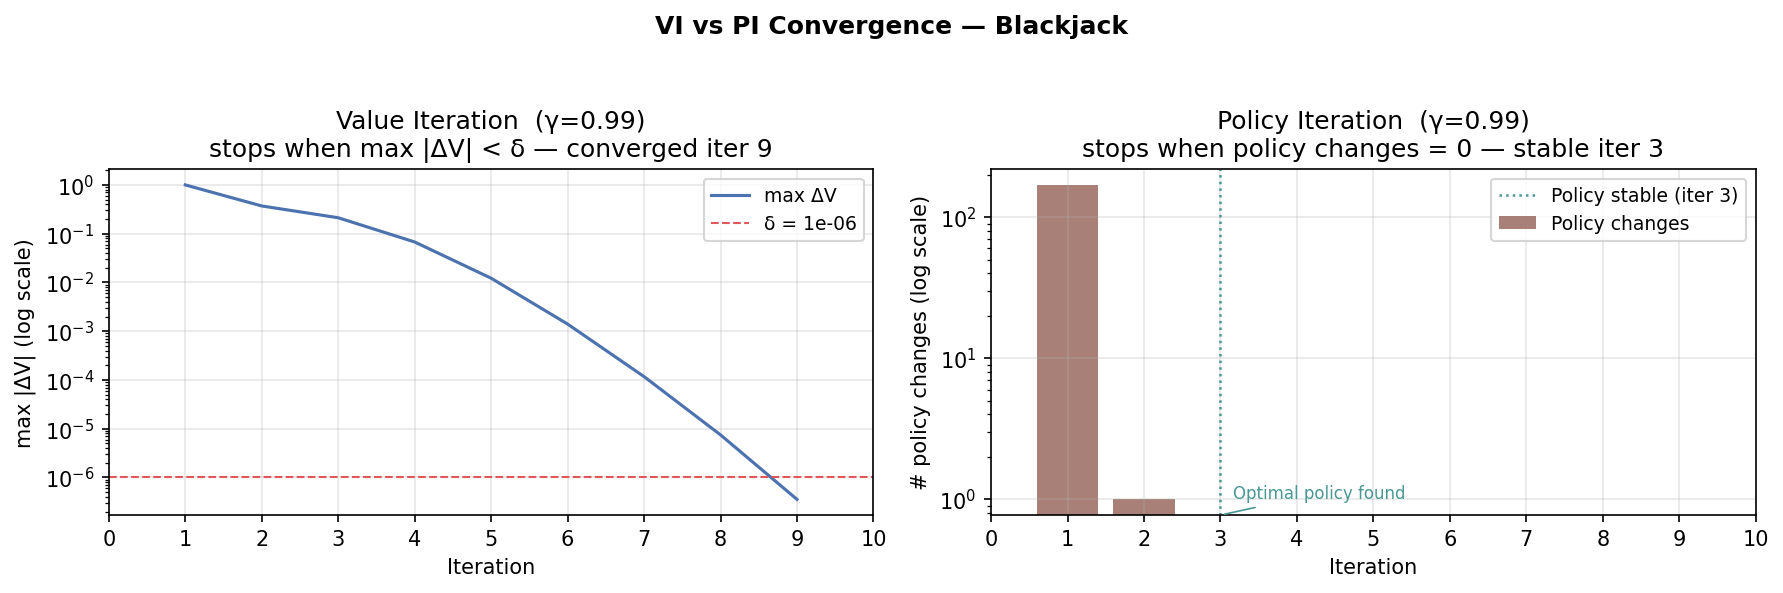
\includegraphics[width=\textwidth]{figures/phase2_vi_pi_blackjack/blackjack_convergence.png}
\caption{Blackjack planning convergence. VI drives the Bellman residual below $10^{-6}$ in 9 sweeps, while PI reaches a stable policy in 3 iterations.}
\label{fig:bj_convergence}
\end{figure*}

The optimal policy is also interpretable. The heatmap in Fig.~\ref{fig:bj_policy} shows the familiar threshold behavior: hard hands stick at high totals, while soft hands tolerate more aggressive hitting because the usable ace softens the bust penalty. The fact that VI and PI recover the same qualitative structure strengthens the claim that the difference between them is computational rather than behavioral on this MDP.

\begin{figure}[t]
\centering
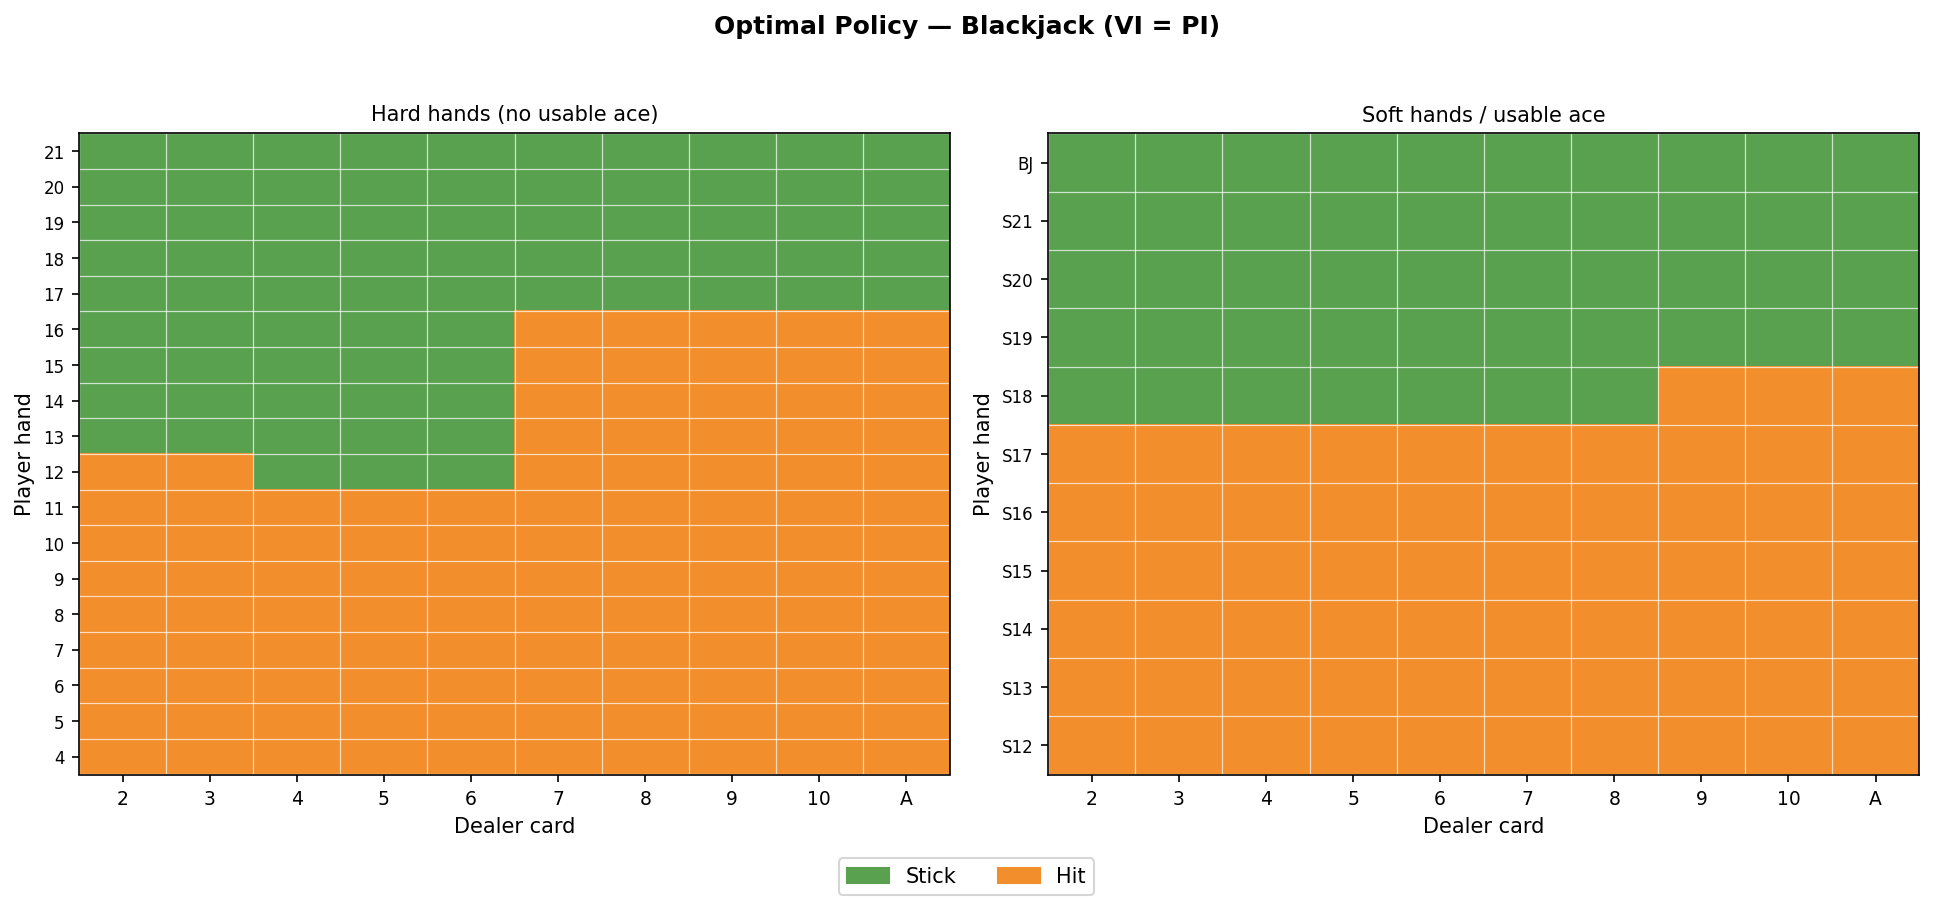
\includegraphics[width=\columnwidth]{figures/phase2_vi_pi_blackjack/blackjack_policy_heatmap.png}
\caption{Blackjack optimal policy recovered by both VI and PI.}
\label{fig:bj_policy}
\end{figure}

\subsection{CartPole: Dynamic Programming and Discretization}

CartPole is more subtle because the fitted model quality depends on the grid. Table~\ref{tab:cp_dp} summarizes the main trade-off. VI required 1376 sweeps on all three grids because the stopping threshold and contraction behavior were nearly identical, but PI needed only 9, 10, and 12 iterations on the coarse, default, and fine grids. The larger differences were in coverage and planning cost. Coverage dropped from \CPCoarseCoverage on the coarse grid to \CPFineCoverage on the fine grid, while fine-grid PI time rose to \CPFinePIWallClock~s.

\begin{figure*}[t]
\centering
\begin{minipage}[t]{0.49\textwidth}
\centering
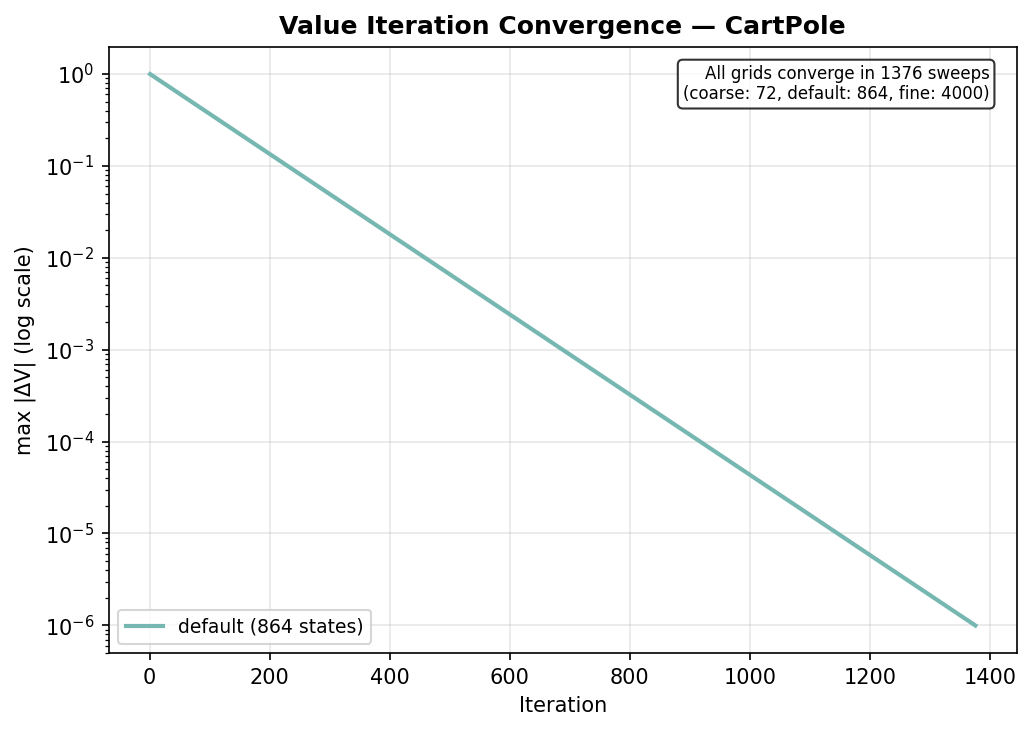
\includegraphics[width=\linewidth]{figures/phase3_vi_pi_cartpole/cartpole_vi_convergence.png}
\end{minipage}\hfill
\begin{minipage}[t]{0.49\textwidth}
\centering
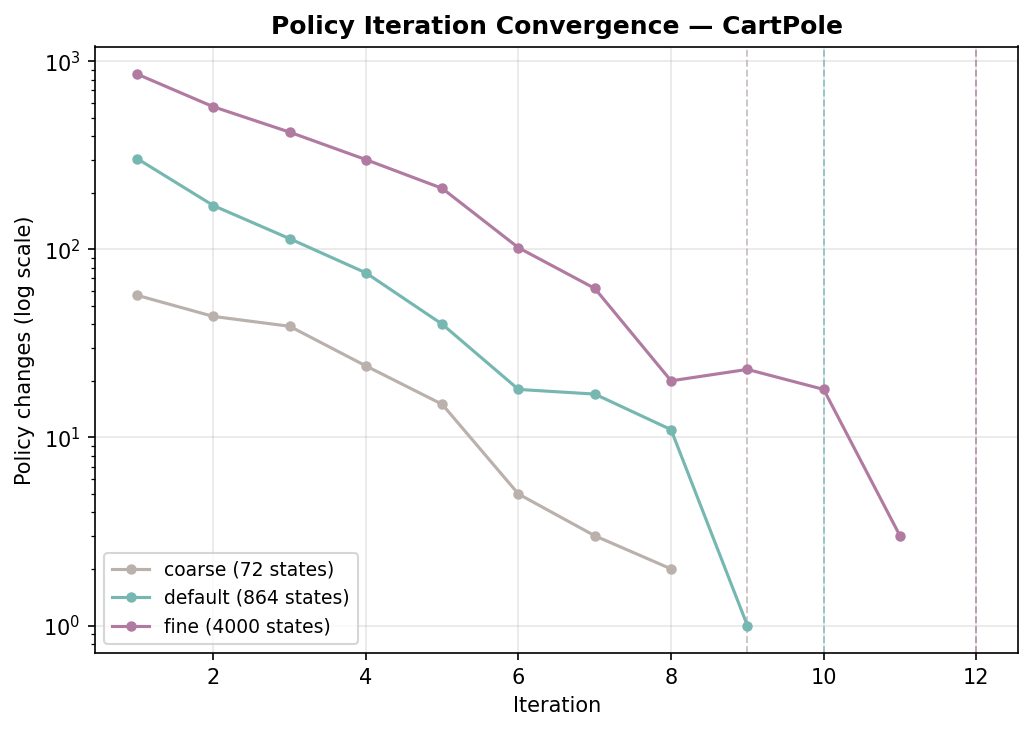
\includegraphics[width=\linewidth]{figures/phase3_vi_pi_cartpole/cartpole_pi_convergence.png}
\end{minipage}
\caption{CartPole planning convergence. VI residual traces overlap across grids, while PI remains much cheaper in iteration count even as the grid is refined.}
\label{fig:cp_dp_convergence}
\end{figure*}

The coarse grid achieved the best evaluation score, including 500-step performance for both VI and PI, but I do not treat that as the most trustworthy representation of the true control problem. With only 72 states and very aggressive aggregation, many physically distinct situations are forced into the same bin. The default grid is a better compromise: it preserves more structure than the coarse model while keeping wall-clock modest (VI \CPDefaultVIWallClock~s, PI \CPDefaultPIWallClock~s). The fine grid pushes in the wrong direction. It expands the state space to 4000 states, coverage collapses, and both performance and runtime deteriorate. For the final algorithm comparison, the default grid is therefore the fairest choice because it avoids both extreme aliasing and extreme sparsity.

\begin{table*}[t]
\caption{CartPole VI/PI summary across discretization grids.}
\label{tab:cp_dp}
\centering
\resizebox{\textwidth}{!}{\begin{tabular}{llrrrrrr}
\hline
\textbf{Grid} & \textbf{Alg.} & \textbf{States} & \textbf{Coverage} & \textbf{Iters} & \textbf{Wall (s)} & \textbf{Ep-len} & \textbf{IQR} \\
\hline
Coarse & VI & 72 & 89.6\% & 1376 & 0.009 & 500.0 & 0.00 \\
 & PI &  &  & 9 & 0.136 & 500.0 & 0.00 \\
\hline
Default & VI & 864 & 25.2\% & 1376 & 0.588 & 456.8 & 5.36 \\
 & PI &  &  & 10 & 0.551 & 465.5 & 1.97 \\
\hline
Fine & VI & 4000 & 16.3\% & 1376 & 16.291 & 434.9 & 3.42 \\
 & PI &  &  & 12 & 50.474 & 436.7 & 3.00 \\
\hline
\end{tabular}
}
\end{table*}

\subsection{Blackjack: SARSA vs. Q-Learning}

Under the shared controlled schedule, SARSA behaved exactly as hypothesized for a stochastic MDP. Its mean return was less negative than Q-learning's (\BJSarsaControlledReturn vs. \BJQLControlledReturn), its final-window variability was lower (0.04 vs. 0.13), and it reached the plateau criterion earlier (\BJSarsaControlledConvEp vs. \BJQLControlledConvEp). The gap persisted after tuning. SARSA improved to \BJSarsaTunedReturn mean return and \BJSarsaTunedConvEp mean convergence episode, while tuned Q-learning still trailed at \BJQLTunedReturn and \BJQLTunedConvEp.

\begin{figure*}[t]
\centering
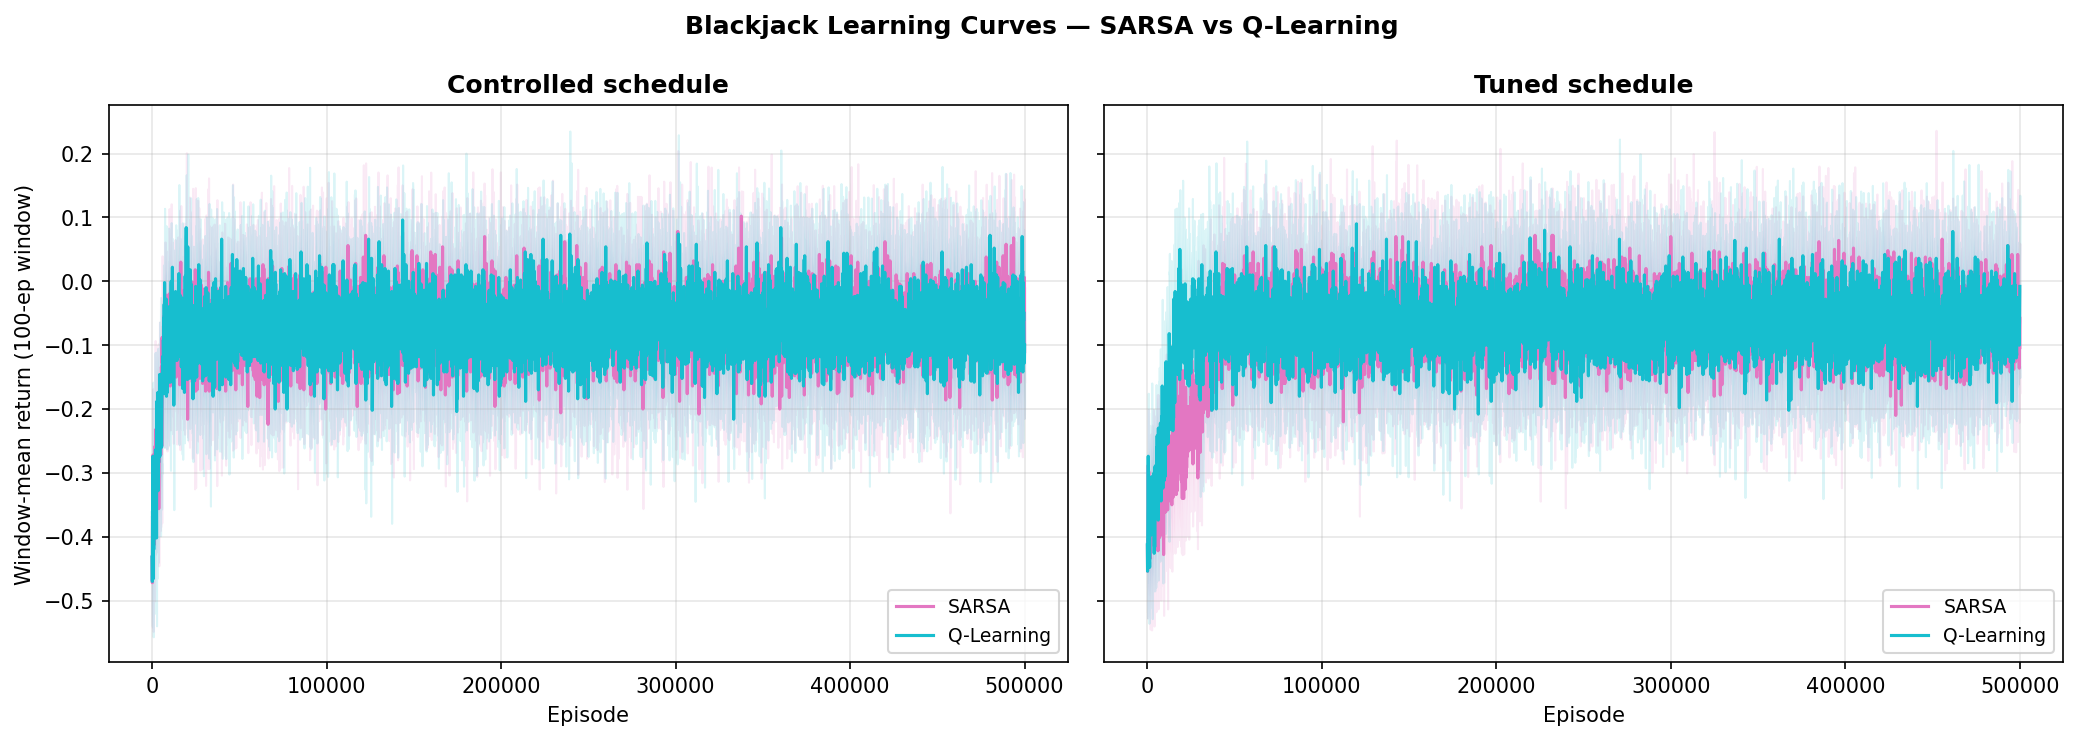
\includegraphics[width=\textwidth]{figures/phase4_model_free_blackjack/blackjack_mf_learning_curves.png}
\caption{Blackjack learning curves under controlled and tuned schedules. Shaded bands show variability across five seeds; SARSA is more stable and reaches better final return on this stochastic task.}
\label{fig:bj_mf_learning}
\end{figure*}

The practical interpretation is that off-policy bootstrapping did not help on Blackjack as much as expected from pure control theory. The stochastic reward structure makes optimistic max targets noisy, and the on-policy SARSA update appears to damp that noise. The hyperparameter search confirmed that exploration schedule mattered more than tiny adjustments to the terminal learning rate: once $\epsilon$ decayed too quickly, both agents locked into mediocre policies, but Q-learning was more sensitive to that failure mode.

\subsection{CartPole: SARSA vs. Q-Learning}

CartPole flips the model-free ranking. Under the controlled schedule, Q-learning already outperformed SARSA (\CPQLControlledEpLen vs. \CPSarsaControlledEpLen mean episode length) while converging at nearly the same episode budget. Tuning widened the gap further: tuned Q-learning reached \CPQLTunedEpLen mean episode length with IQR \CPQLTunedEpLenIQR, while tuned SARSA reached \CPSarsaTunedEpLen with IQR \CPSarsaTunedEpLenIQR.

\begin{figure*}[t]
\centering
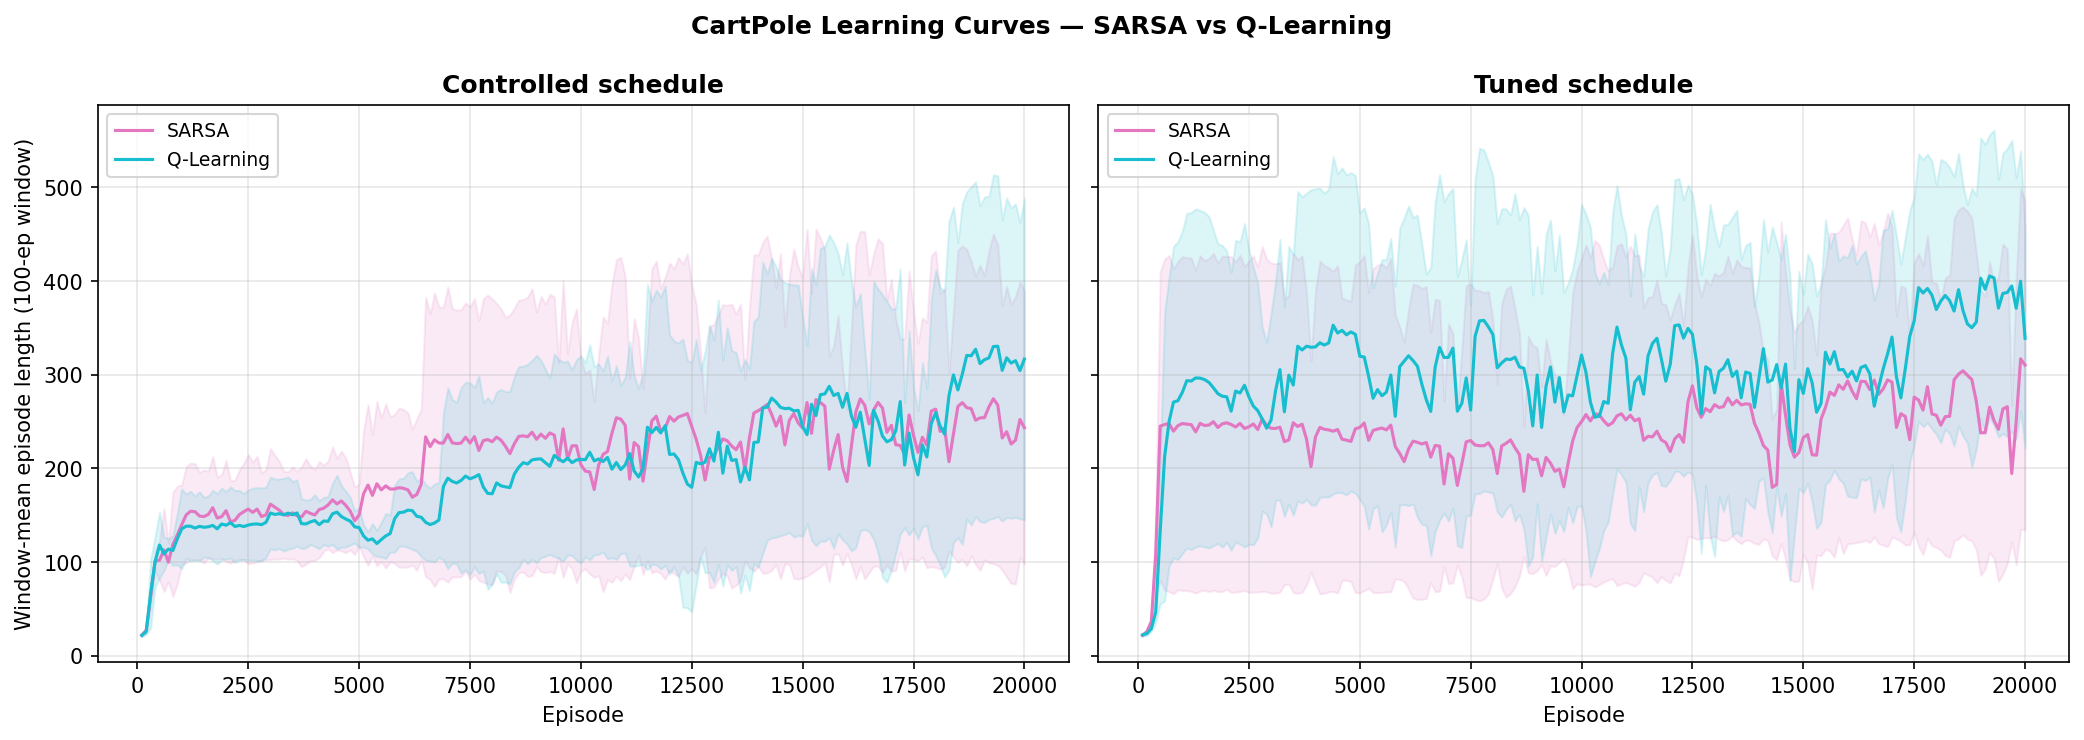
\includegraphics[width=\textwidth]{figures/phase5_model_free_cartpole/cartpole_mf_learning_curves.png}
\caption{CartPole learning curves under controlled and tuned schedules. Shaded bands show variability across five seeds; Q-learning benefits more from tuning on the default grid.}
\label{fig:cp_mf_learning}
\end{figure*}

The discretization ablation in Table~\ref{tab:cp_disc} shows the same coarse/default/fine pattern observed in DP. The fine grid is too sparse for stable tabular learning and both algorithms collapse badly there. The coarse grid is strongest numerically, especially for Q-learning, but again it achieves that strength with much stronger aliasing. The default grid remains the best balanced choice for report-wide comparisons because it is expressive enough to model the pole-angle dynamics while still receiving enough repeated visits for robust learning.

\begin{table}[t]
\caption{CartPole tuned-regime discretization study.}
\label{tab:cp_disc}
\centering
\resizebox{\columnwidth}{!}{\begin{tabular}{lrr}
\hline
\textbf{Grid} & \textbf{SARSA Ep-len} & \textbf{Q-Learning Ep-len} \\
\hline
Coarse & 364.3 & 438.1 \\
Default & 325.3 & 376.8 \\
Fine & 94.6 & 110.3 \\
\hline
\end{tabular}
}
\end{table}

\subsection{Cross-Method Synthesis}

The cross-method view makes two points clear. First, PI is computationally preferable to VI whenever both are available. It reduces planning iterations from 9 to 3 on Blackjack and from 1376 to 10 on default-grid CartPole while preserving or slightly improving final performance. Second, dynamic programming remains strongest overall on these small-to-medium MDPs. On Blackjack, VI and PI both outperform the tuned model-free agents in final return. On CartPole, DP on the default grid still beats tuned Q-learning by a large margin (PI \CPDefaultPIEpLen, VI \CPDefaultVIEpLen, tuned Q-learning \CPQLTunedEpLen).

\begin{figure*}[t]
\centering
\begin{minipage}[t]{0.49\textwidth}
\centering
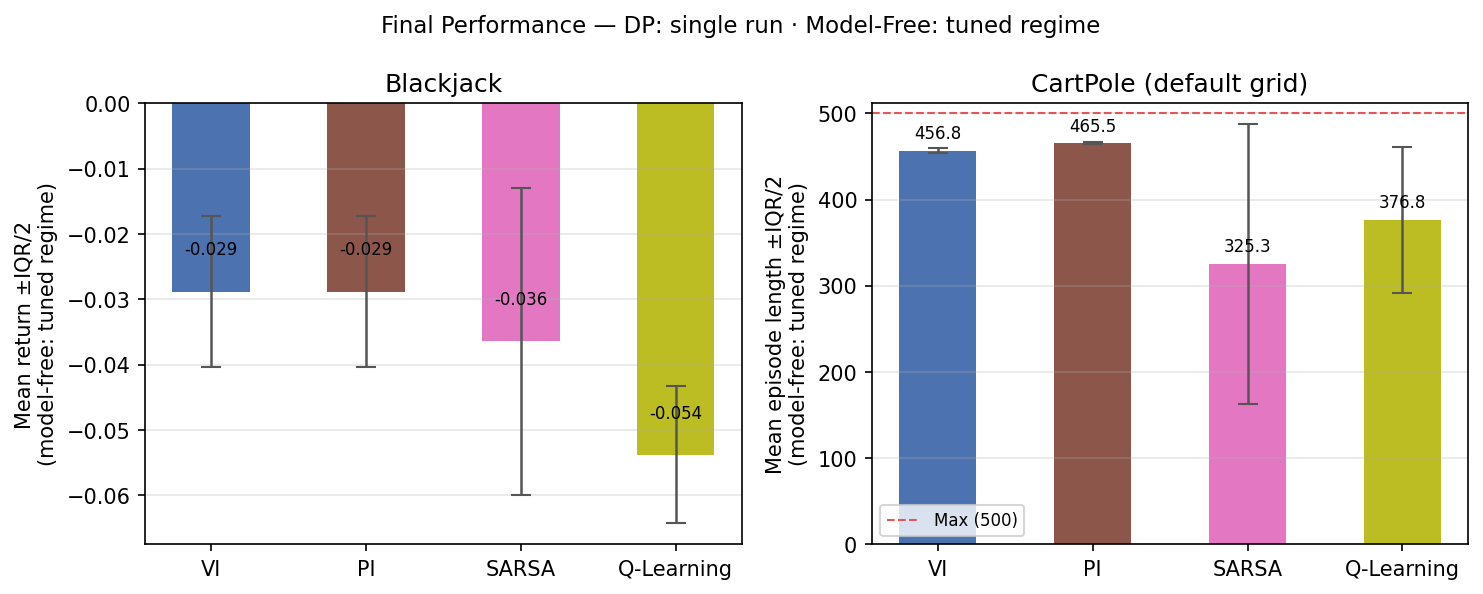
\includegraphics[width=\linewidth]{figures/phase6_comparison/final_performance_comparison.png}
\end{minipage}\hfill
\begin{minipage}[t]{0.49\textwidth}
\centering
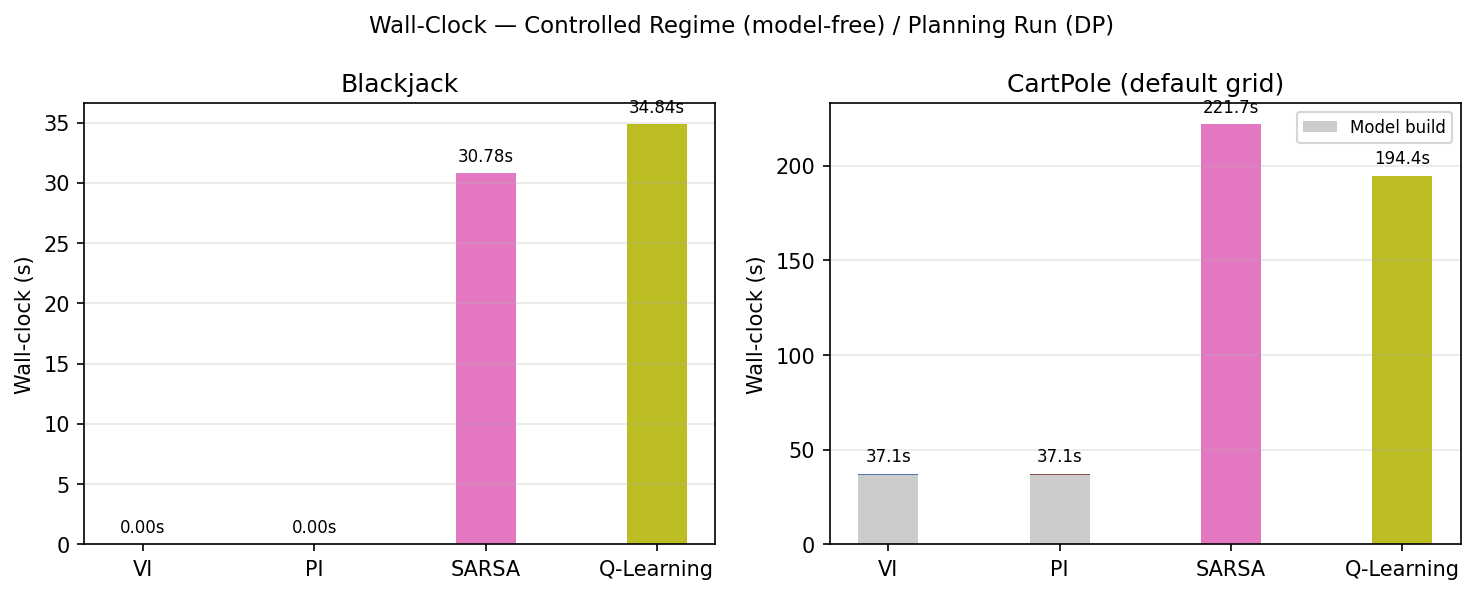
\includegraphics[width=\linewidth]{figures/phase6_comparison/wall_clock_comparison.png}
\end{minipage}
\caption{Cross-method summary. Left: final performance using tuned model-free agents and the default CartPole grid. Right: wall-clock cost under the controlled regime. On CartPole, the model-build overhead is real but still cheaper than the final model-free training runs.}
\label{fig:cross_method}
\end{figure*}

The wall-clock result is important because it moderates the usual claim that model-based planning is only attractive on tiny problems. On Blackjack, planning time is effectively zero. On CartPole, the learned model costs \CPModelBuildWallClock~s to build, but the total DP runtime is still only about 37~s, compared with \CPSarsaWallClock~s and \CPQLWallClock~s for the controlled model-free runs. On this assignment, a decent model is worth the upfront cost.

\subsection{Extra Credit: Vanilla DQN vs. Double DQN}

For extra credit, I implemented a small replay-based DQN with a 64-unit hidden layer, replay buffer size 10,000, batch size 64, target-network refresh every 500 steps, and 2000 training episodes. Unlike tabular Q-learning, which stores a separate value for each discrete state-action pair, DQN learns a neural approximation to $Q(s,a)$ and stabilizes training with replay memory and a delayed target network. I then compared a vanilla target against a Double DQN target, where Double DQN decouples action selection from target evaluation to reduce overestimation. The result is mixed rather than triumphant. Vanilla DQN reached \VanillaDQNEvalEpLen greedy-evaluation mean episode length, Double DQN reached only \DoubleDQNEvalEpLen, and neither variant satisfied the convergence rule within the 2k-episode budget. Tuned tabular Q-learning remained strongest at \DQNQLBaseline.

\begin{table}[t]
\caption{Extra-credit DQN summary on CartPole.}
\label{tab:dqn}
\centering
\resizebox{\columnwidth}{!}{\begin{tabular}{lrrr}
\hline
\textbf{Method} & \textbf{Greedy Eval Ep-len} & \textbf{IQR} & \textbf{Converged (2\,k ep)} \\
\hline
Vanilla DQN & 351.6 & 335.9 & No \\
Double DQN & 226.4 & 124.8 & No \\
\hline
\textit{Tuned SARSA} & 325.3 & 323.7 & -- \\
\textit{Tuned Q-Learning} & 376.8 & 169.1 & -- \\
\hline
\end{tabular}
}
\end{table}

The main lesson is that function approximation did not automatically improve this problem. Vanilla DQN was competitive with tuned SARSA, but it did not beat tuned tabular Q-learning, and Double DQN was worse than vanilla in the current compute budget. That is a useful result: the gap between tabular control and neural control is not just representational capacity, but also optimization stability, replay quality, and training horizon.

\section{Conclusion}

The experiments largely support the original hypothesis, but with one important refinement. PI is clearly the more efficient planner than VI on both tasks, and model-based methods dominate final performance whenever the model is reliable enough. On Blackjack, that dominance is complete because the model is exact. On CartPole, the choice of grid matters as much as the choice of algorithm. Both dynamic programming and tabular control degrade when the grid becomes too fine for the available coverage, while the coarse grid can look stronger than it really is because of aggressive aliasing. Under that constraint, the default grid is the best compromise for fair cross-method comparison.

Among model-free agents, SARSA is the safer choice on stochastic Blackjack, while tuned Q-learning is better on discretized CartPole. The extra-credit DQN study reinforces the same theme: more expressive function approximation is not automatically better when the training budget is short and the task is already solvable with a strong tabular baseline. Overall, the project shows that environment structure, abstraction quality, and update target matter at least as much as the algorithm family name.

\section*{AI Use Statement}

I used GitHub Copilot and chat-based coding assistance to brainstorm report structure, refactor and debug parts of the experiment code, and improve wording and organization in the write-up. I reviewed, verified, and understand all assisted content, and all numerical claims in this draft were checked against the generated experiment outputs, local figure copies, and LaTeX tables.

\section*{References}

References and in-text citations are intentionally omitted in this working draft and will be added in the final pass.

\end{document}
